\section{Experimental Methods and Time Series Explanations}

\subsection{Time Series Collection}
 Experimental methods (how we collect the time series and what the times series are
This should be HPM PAPI, which programs we model


\subsection{The Programs}
Include traces of full \col \svd and \gcc
\begin{figure}[htbp]
  \centering
  \begin{subfigure}[t]{0.475\textwidth}
    \includegraphics[width=0.95\textwidth]{figs/colFullTS}
    \caption{\col Time Series}
    \label{fig:col-ts}
  \end{subfigure}%
  \begin{subfigure}[t]{0.475\textwidth}
    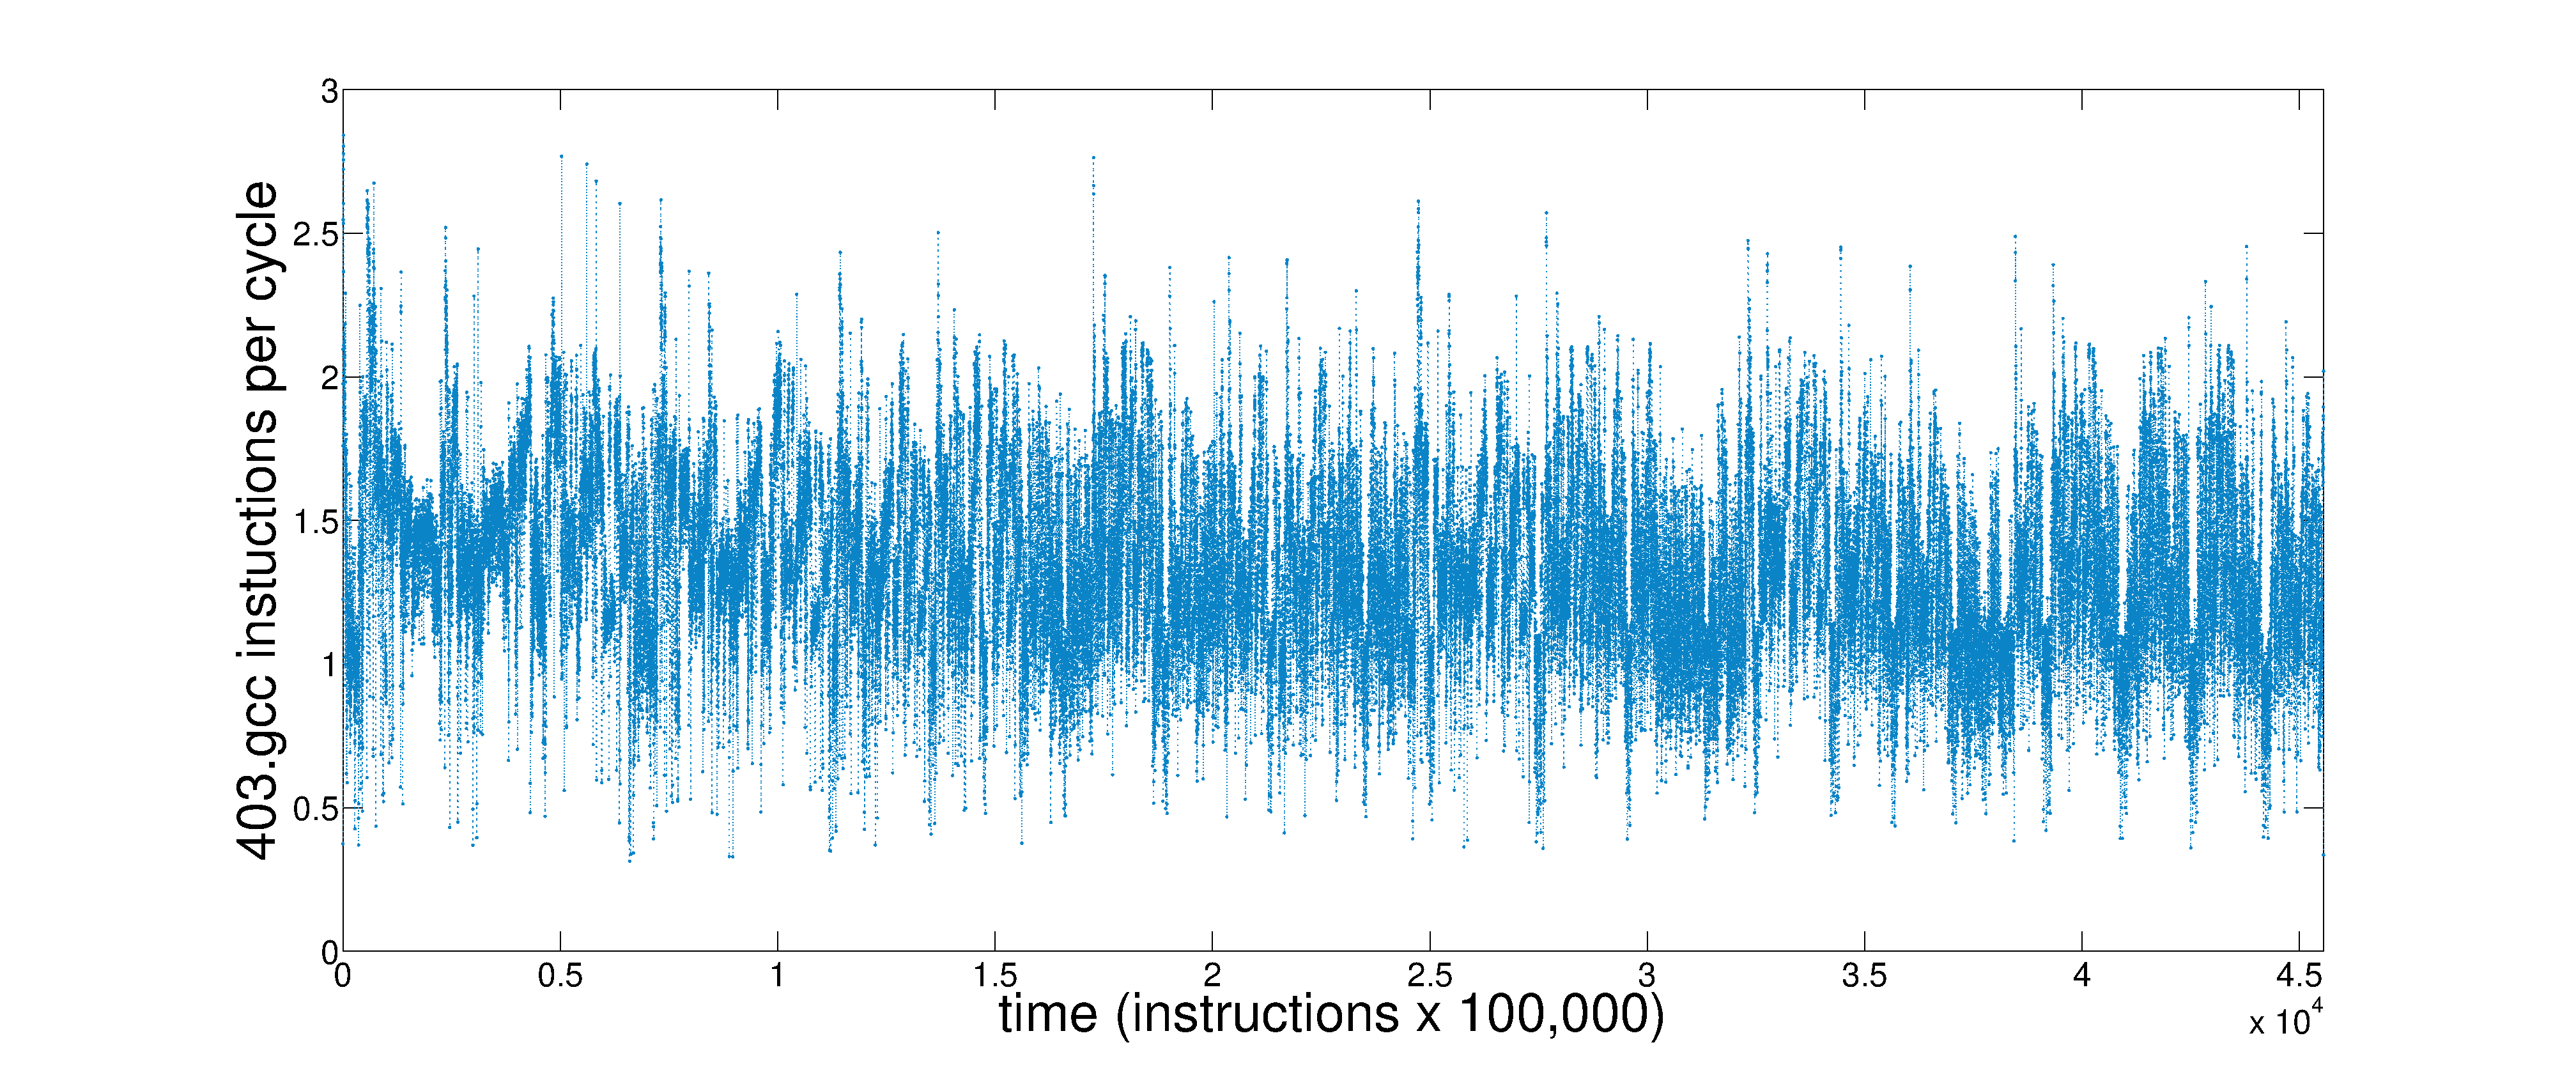
\includegraphics[width=0.95\textwidth]{figs/gccfullts}
    \caption{\gcc Time Series}
    \label{fig:gcc-ts}
  \end{subfigure}
    \begin{subfigure}[t]{0.475\textwidth}
    \includegraphics[width=0.95\textwidth]{figs/SVD1RegimesColored}
    \caption{\svd Time Series with Regime Coloring}
    \label{fig:svd-ts-colored}
  \end{subfigure}
  \caption{[[Maybe this should be just a picture of each time series and then have another figure with color after explaining heuristically the reigmes. In (a) the instructions executed per CPU clock cycle
    (IPC) during the execution of \col. Each point is the average IPC during a 100,000
    instruction period. Similarly in (b) is a time series of the IPC during the execution of \gcc.}\label{fig:sample-ts}
    \end{figure}

\svd brings up a very interesting point: systems change over time. While it is clear in Figure \ref{fig:sample-ts} (a) and (b) that a single system is being observed, it also appears \emph{visually} that the complexity of these two time series is consistent over time, i.e., while they are both complicated they don't appear to increase or decrease in complexity over the range of the program. \svd (seen in Figure \ref{fig:svd-ts-colored}) is different however, at least visually. Figure \ref{fig:svd-ts-colored} is a single trace of \svd from start to finish, however as time progresses it is clear that something drastically changes in the underlying generating process and the structure of the time series is visually very different from section to section. This is caused by the code of \svd moving between different subroutines. We call these changes in \svd dynamics  \emph{\svd regimes} and we have colored each of the six regimes different colors in Figure \ref{fig:svd-ts-colored}. The advantage to splitting \svd into these regimes is to explore how complexity and predictability evolve over time for a system in drift. In Section \ref{sec:wpeRegime} we explore and validate the choice of these visually selected regime windows extending techniques from \cite{cao2004det}. The purpose of this paper is not to rigorously explore regime detection but to explore quantifying complexity of a time series. As such, making this split simply serves as providing 90 unique time series\footnote{Six Regimes with 15 individual runs each.} to explore. For notational convience we refer to these signals as {\tt dgesdd$_i$} with $i \in \{1\dots6\}$ where $i$ corresponds to a regime of \svd. The regimes are labeled from left to right. 


